\documentclass{article}
\usepackage[final, nonatbib]{"neurips_2020"}
\usepackage[utf8]{inputenc} % allow utf-8 input
\usepackage[T1]{fontenc}    % use 8-bit T1 fonts
\usepackage{hyperref}       % hyperlinks
\usepackage{url}            % simple URL typesetting
\usepackage{booktabs}       % professional-quality tables
\usepackage{amsfonts}       % blackboard math symbols
\usepackage{nicefrac}       % compact symbols for 1/2, etc.
\usepackage{microtype}      % microtypography
\usepackage{xcolor}         % colors
\usepackage[
style=authoryear,
backend=bibtex,
]{biblatex}
\bibliography{finalbib}
\usepackage{graphicx}
\graphicspath{ {./Graphics/} }
\usepackage{easytable}
\usepackage{enumitem}
\usepackage{placeins}
\usepackage{float}


\title{Image Classification Experiments for Landmarks Around the World}
\author{Adam Dameron, Anthony Kayode, Vivian Moore, David Peery}


\begin{document}
	
	
\maketitle
	
\begin{abstract}
	This paper seeks to provide an understanding of how three different models perform on an image classification task. These models are pre-trained, and transfer learning will be used to allow them to work with the dataset in question. Code of the project is available at \url{https://github.com/Adameron0/STOR-566-Project}
\end{abstract}

\section{Introduction}

According to a Pew Research survey, dating apps like Tinder and Bumble are an increasingly popular way for people to connect and meet with like-minded individuals, with 3/10 adults in the US reporting having used some dating site/app. This same survey asserts that 26\% of Americans believe that online dating has a negative effect on dating and relationships, and of that 26\%, 14\% cited the lack of personal/emotional connections as their primary reason (Anderson et al.). When considering how these apps could alleviate some of the negative stigma surrounding them, algorithmic improvements appeared promising. 

A 2017 study conducted by Hinge found that travel photos receive 30\% more likes than the average photo a user uploads (Shrikant). With this proclivity toward travel photos in mind, we hypothesized that if these apps used these travel photos as an additional factor when curating matches, users could be connected with more like-minded individuals on the basis of shared experiences. For example, a user’s photo of the Eiffel Tower could be used to match them with other people who have visited France or share an appreciation for French culture.

The goal of this project is to compare the performance of different pre-trained image classification models on the Wonders of the World dataset in order to determine which model a company like Match Group might want to implement on their backend.


\section{Related Works}

There are a plethora of papers that have been published with the goal of comparing different image classification models on a dataset using transfer learning. Before explaining some of these papers, it is worth noting that the majority of them do not evaluate the two newer image classifier models we chose to use in our experiment \parencite{vit, cvt}, which makes sense given the recent release of these models. For brevity’s sake, this section will describe two papers that shared a similar objective with our experiment. In the paper, “A Comparative Study of Deep Learning-based Image Classification Models for Material Classification,” the authors tested various image classification models to see which one would be able to best classify images of materials like paper or plastic \parencite{Gokhale}. Similar to our experiment, they chose three pre-trained image classification models for comparison. The models they used were the VGG-16, ResNet-50 (which is one of the models we used), and the Inception v3 \parencite{Gokhale}. Using an SGD optimizer for each of their models, they found that the VGG-16 model outperformed the ResNet-50 and Inception v3 for validation accuracy, with Inception v3 significantly underperforming when compared to the other two \parencite{Gokhale}. Thus, the authors found that the VGG-16 pre-trained model was the best at classifying images of materials out of the three pre-trained models that were analyzed.

Another paper that shared a similar objective with our experiment was the paper, “Comparison of Convolutional Neural Networks Model Using Different Optimizers for Image Classification.” The goal of this paper was to evaluate which pre-trained image classifier model would be best at predicting gender \parencite{Wirayasa}. The authors of this paper experimented with the VGG-16 model, the Inception v3 model, and the MobileNet-v2 model \parencite{Wirayasa}. Using the AdamW optimizer and RMS prop, they obtained results that were quite different from the paper described above. The Inception v3 model had the highest accuracy when it came to predicting gender, with VGG-16 trailing closely behind \parencite{Wirayasa}. The stark difference in results between these two papers speaks to how the effectiveness of deep learning models can depend on the dataset they are trained and evaluated on. While the paper that aimed to determine which model would be able to best classify materials showed that the Inception v3 model had the worst performance, the paper that aimed to show which model would be best at classifying gender found that the Inception v3 model had the best performance. Based on the conflicting results from these papers about which model performs best, it becomes all the more necessary to evaluate multiple models on our dataset to determine which model will work best.

\section{Proposed Methods}

\subsection{Overall Description}

There were two parts to our experiment. The first part evaluated which of the three pre-trained models selected (ResNet-50, ViT, or CvT) would perform best on our dataset without any data augmentation. The second part evaluated which of these same three pre-trained models would perform best on our dataset using data augmentation techniques. The reason why we wanted to evaluate these models both with and without data augmentation is because of the size of our dataset. The dataset is very small, so our group initially suspected that there would be a problem with overfitting. We wanted to see if data augmentation would mitigate any potential overfitting problems with the models that we were experimenting with.

To evaluate which of the three models (ResNet-50, ViT, CvT) would perform best on the Wonders of the World dataset, the first step of this experiment was to obtain each model using HuggingFace. HuggingFace is an open-source platform where machine learning models can be downloaded for training and deployment. In the case of this experiment, the ResNet-50 model from Microsoft, the vit-base-patch16-224 from Google, and the cvt-13 from Microsoft and their respective pre-trained weights were all obtained from HuggingFace. 

\subsection{Model Descriptions}

\subsubsection*{Residual Neural Networks}

The first model used for this series of experiments was the ResNet-50. This model was based on the paper “Deep Residual Learning for Image Recognition”, which was written in 2015. The paper sought to address the degradation problem, which occurs when training error increases as the depth of a neural network increases (He, et al.). To tackle this problem, the authors developed a residual neural network using shortcut connections to perform identity mapping (He, et al.). These identity mappings would allow for the model to retain more information from the previous layer (He, et al.). The architecture of the ResNet-50 model obtained from HuggingFace differed slightly from that of the model in the paper. It has a stride of 2 in the 3x3 convolution instead of the first 1x1 convolution (Microsoft/Resnet-50). The model was pre-trained on the ImageNet-1k dataset (Microsoft/Resnet-50).

\subsubsection*{Vision Transformer}

The next model that was used for the experiments was the Vision Transformer (ViT). This model was based on the paper “An Image Is Worth 16x16 Words: Transformers for Image Recognition at Scale”,  which was written in 2020. The authors of this paper argued that a reliance on CNNs for image classification is not necessary and that a transformer-based model architecture (usually used for tasks like NLP) can be applied to image classification tasks (Dosovitskiy, et al.). To show this, the authors developed a transformer architecture, in which the image was broken into 16x16 patches, each of the resulting patches was linearly embedded, position embeddings were added, and the resulting sequence of vectors was fed to a transformer encoder (Dosovitskiy, et al.). They also added a classification token to the sequence for the classification task. The architecture of the model for the ViT taken from HuggingFace is the exact same as that of the model taken from the paper. The model was pre-trained on the ImageNet-21k dataset (Google/VIT-Base-patch16-224.).

\subsubsection*{Convolutional Vision Transformer}


The final model that was evaluated was the Convolutional Vision Transformer (CvT), which was developed in 2021. This model was based on the paper “CvT: Introducing Convolutions to Transformers”, which sought to address some of the shortcomings of the ViT. Specifically, the authors noticed that while larger ViT models may be able to outperform large CNNs, the smaller-scale ViT models were still unable to outperform CNN counterparts of a similar size (Wu, et al.). The authors believed that this was because the ViT architecture lacked certain desirable properties of a CNN (Wu, et al.). To modify the ViT architecture so that it would incorporate some CNN properties, the authors made two key changes to the architecture. A hierarchy of transformers was developed through a convolutional token embedding to give the model a hierarchical structure that closely resembles that of CNNs (Wu, et al.). Additionally, a convolutional transformer block leveraging a convolutional projection replaced the original transformer block of the ViT to give the ViT certain properties of a CNN, such as receptive fields, shared weights, and spatial subsampling (Wu, et al.). The CvT model obtained from HuggingFace has the same architecture as the one described in the paper. The model was pre-trained on the ImageNet-1k dataset (Microsoft/CVT-13).

\subsection{Data Procedures}

For further training and validation of the models on the Wonders of the World dataset, the dataset was split into training and validation using a 95/5 ratio. The reason why the validation set only consisted of 5\% of the data (as opposed to a larger percentage like 10\% or 20\%) was that the dataset itself was very small, and we wanted to have as much training data as possible. It should also be noted that the size of the training and validation data was the same for each class (each one having exactly 150 training images and 8 validation images). After splitting the data, a dataset class was created, where the pixel data and label for each image were obtained. It was also in this class that each of the images was resized to 16x16 pixels for training purposes (training and validating each of the full-size images for 20 epochs would be highly computationally expensive). The training and validation sets were then run through the PyTorch DataLoader function. Both the training and validation sets were batched into groups of eight, and the training data was shuffled.

\subsection{Experimental Procedures}

For the first half of the experiment, the models were trained and validated without any data augmentation, other than resizing the image. Each of the pre-trained models was loaded. The loss function was consistent across all three models, which was the Cross-Entropy Loss function from PyTorch (the suggested loss function for multi-class classification). The optimizer tested on all three models was the AdamW optimizer from PyTorch, and the hyperparameters used for this optimizer across all three models were as follows; weight decay = 0.0001 and learning rate = 0.0001. Each model was trained and validated for 20 epochs using the GPU available on Google Colab, and the training loss, training accuracy, validation loss, and validation accuracy were recorded at the end of each epoch for model comparison purposes. 

For the second half of our experiment, we augmented the data and re-trained/re-validated the three models. To augment the data, we added two transformations to our dataset class before running it through the DataLoader. The first augmentation was a random rotation of 180 degrees, where the image was rotated by 180 degrees. The second augmentation was a gaussian blur, which blurred the image. These were then wrapped in the transforms.Compose function to allow the transformations to be applied to the images sequentially. This allowed for the batch images to be copied and transformed with every iteration, which augmented our dataset to allow the model to see more training and validation images during each epoch. All three pre-trained models and their respective weights were once again loaded. Similar to the first half of the experiment, Cross Entropy Loss was chosen as the loss function and the AdamW optimizer was used (with weight decay set to 0.0001 and learning rate set to 0.0001 again), and each model was once again trained and validated for 20 epochs using the GPU available on Google Colab, where the training loss, training accuracy, validation loss, and validation accuracy were recorded. The purpose of the second half of this experiment was to see how the loss and accuracy results from the testing and validation sets changed after the data was augmented to offset potential overfitting.

\section{Experiments}


\FloatBarrier
\begin{table}
	\begin{center}
		\caption{Experiments Without Data Augmentation}
		
		\begin{tabular}{|c|c|c|}
			% <-- Alignments: 1st column left, 2nd middle and 3rd right, with vertical lines in between
			\hline
			\rule{0pt}{20pt}
			\textbf{Model} &       \textbf{Loss Plot}       &     \textbf{Accuracy Plot}     \\ \hline
			\rule{0pt}{80pt}
			  ResNet-50    & 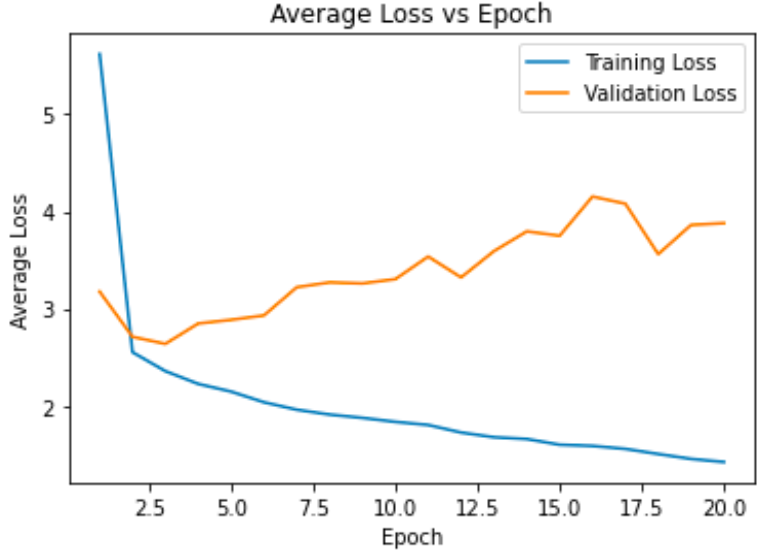
\includegraphics[width=2in, height = 1in]{1} & 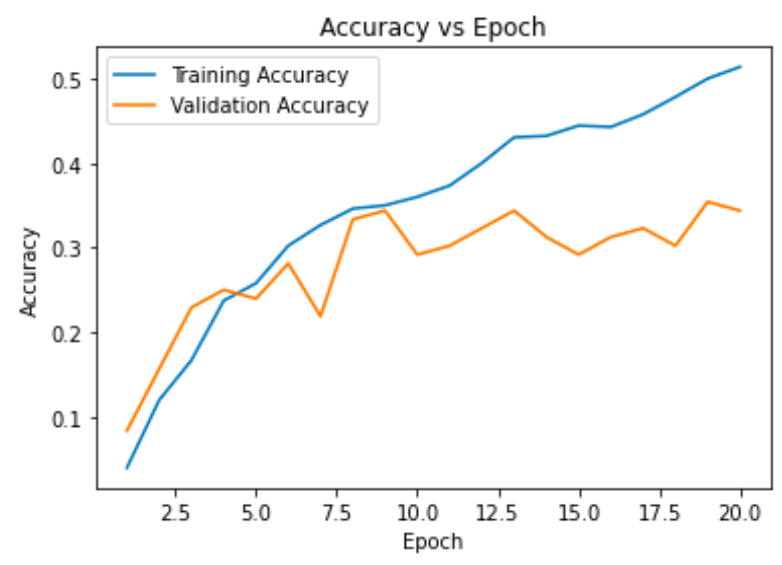
\includegraphics[width=2in, height = 1in]{2} \\ \hline
			  \rule{0pt}{80pt}
			     ViT       & 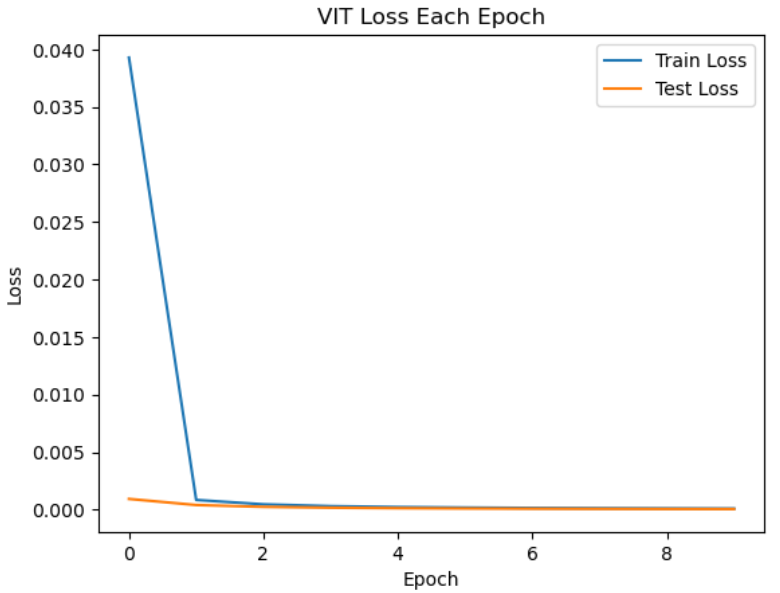
\includegraphics[width=2in, height = 1in]{3} & 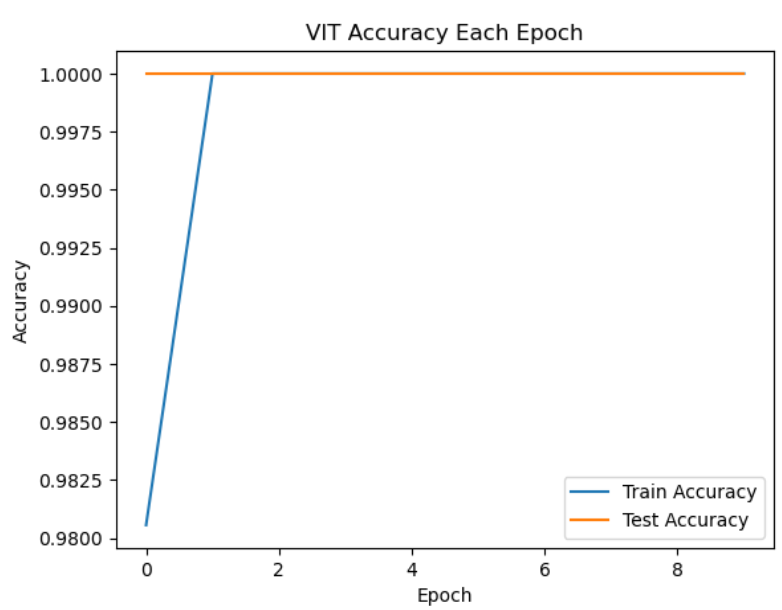
\includegraphics[width=2in, height = 1in]{4} \\ \hline
			     \rule{0pt}{80pt}
			     CVT       & 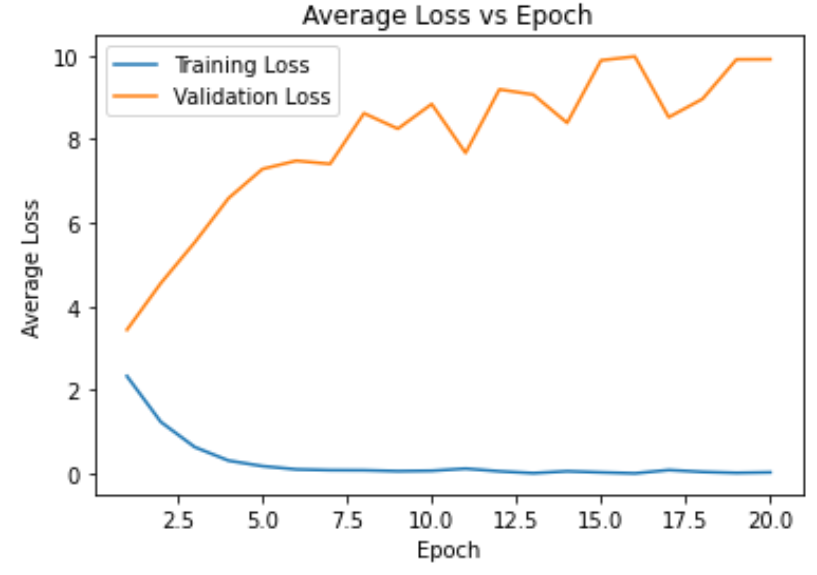
\includegraphics[width=2in, height = 1in]{5} & 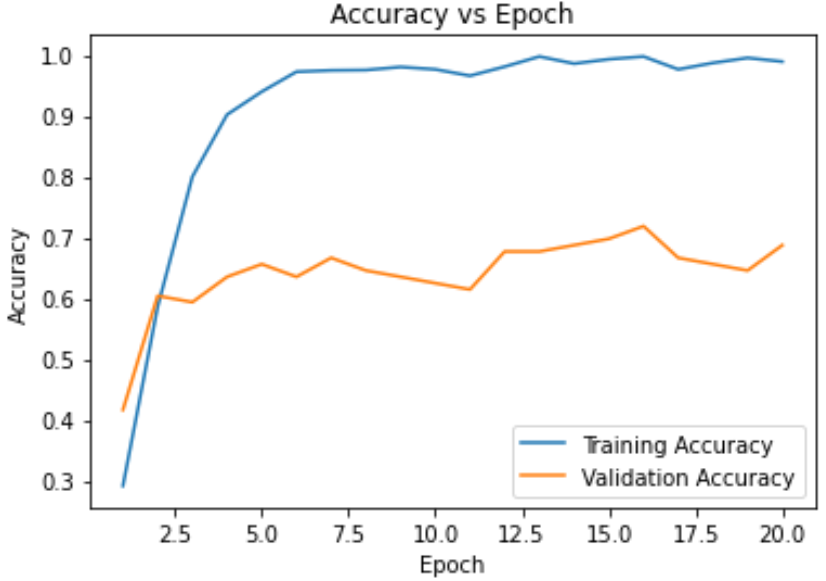
\includegraphics[width=2in, height = 1in]{6} \\ \hline
			     
		\end{tabular}
	\end{center}
\end{table}

For the Resnet and CvT models, we had a clear problem with overfitting. As those models learned, the training accuracy became much higher than the validation accuracy, and the training loss became much lower than the validation loss. In fact, in the CvT model, the validation loss actually continued to increase throughout training. We anticipate that this overfitting was largely due to our relatively small dataset.


\begin{table}[h!]
	\begin{center}
		\caption{Experiments With Data Augmentation}
		
		\begin{tabular}{|c|c|c|}
			% <-- Alignments: 1st column left, 2nd middle and 3rd right, with vertical lines in between
			\hline
			\rule{0pt}{20pt}
			\textbf{Model} &       \textbf{Loss Plot}       &     \textbf{Accuracy Plot}     \\ \hline
			\rule{0pt}{80pt}
			ResNet-50    & 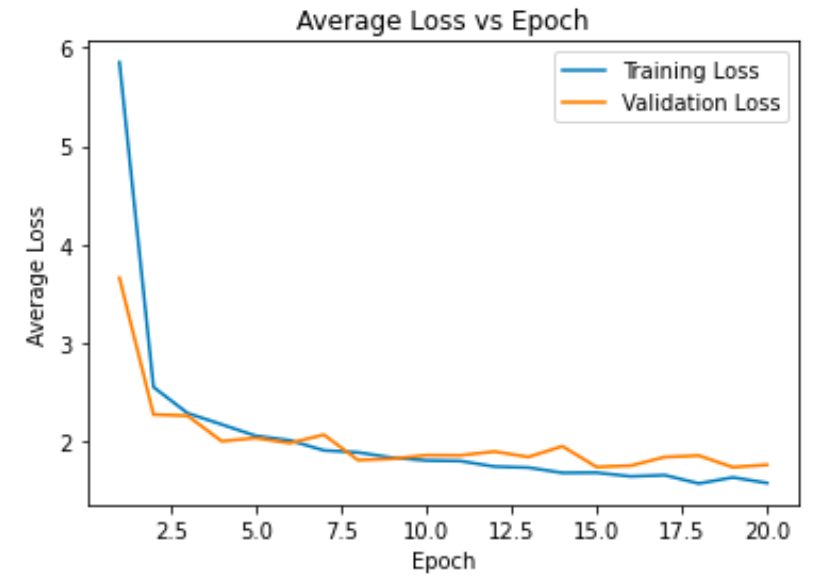
\includegraphics[width=2in, height = 1in]{7} & 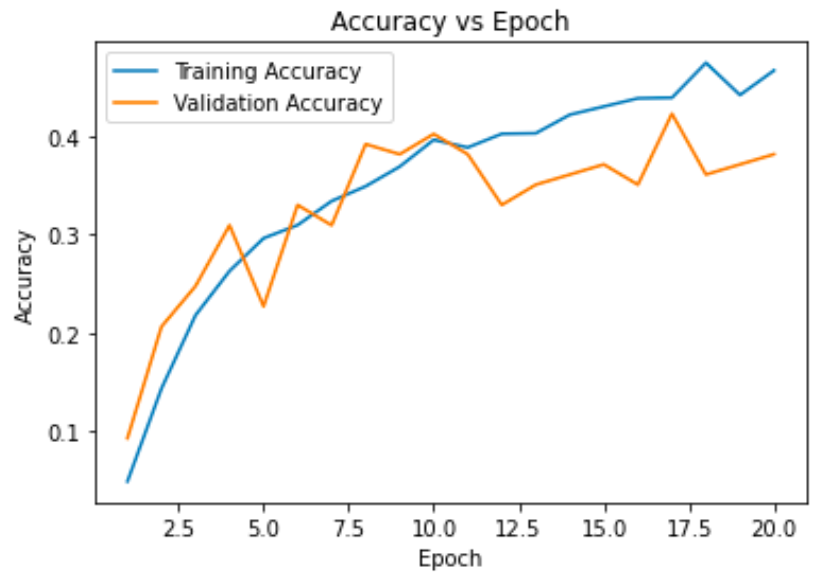
\includegraphics[width=2in, height = 1in]{8} \\ \hline
			\rule{0pt}{80pt}
			ViT       & 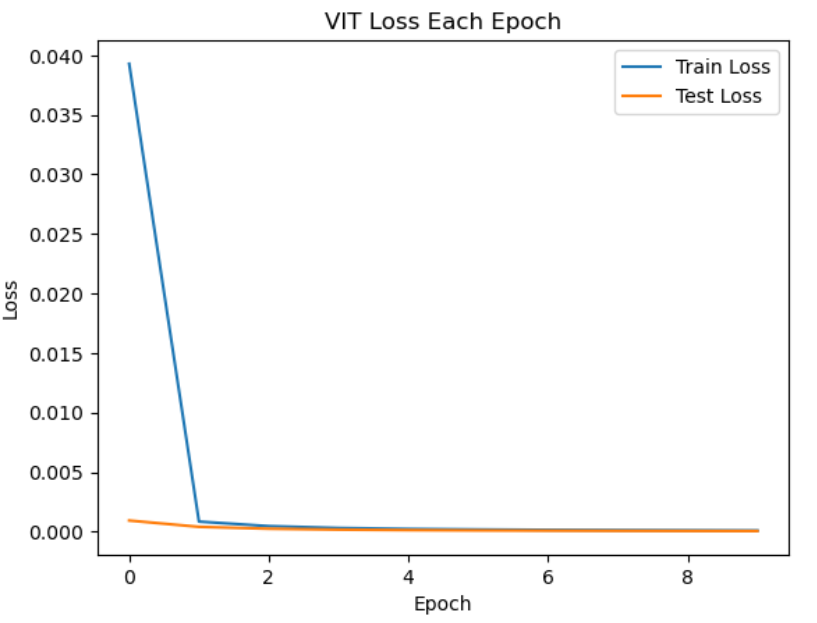
\includegraphics[width=2in, height = 1in]{9} & 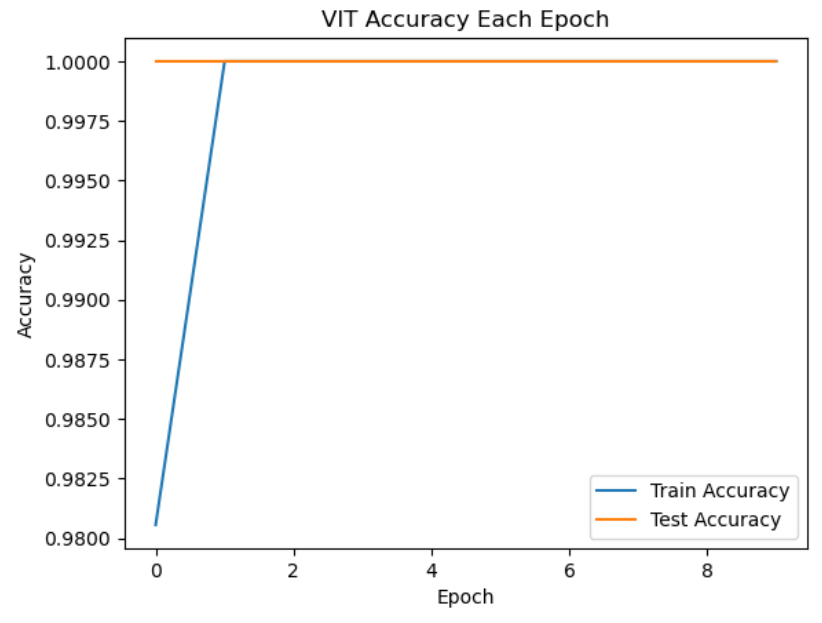
\includegraphics[width=2in, height = 1in]{10} \\ \hline
			\rule{0pt}{80pt}
			CVT       & 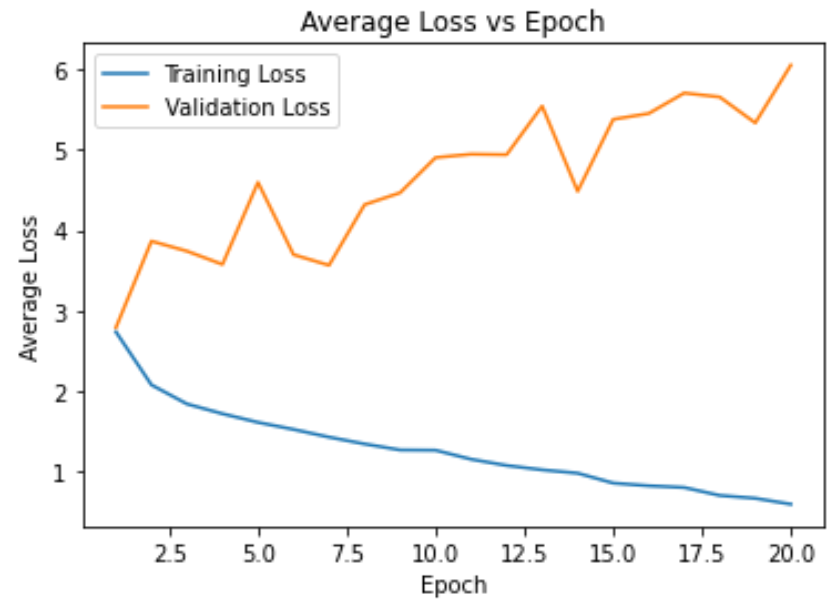
\includegraphics[width=2in, height = 1in]{11} & 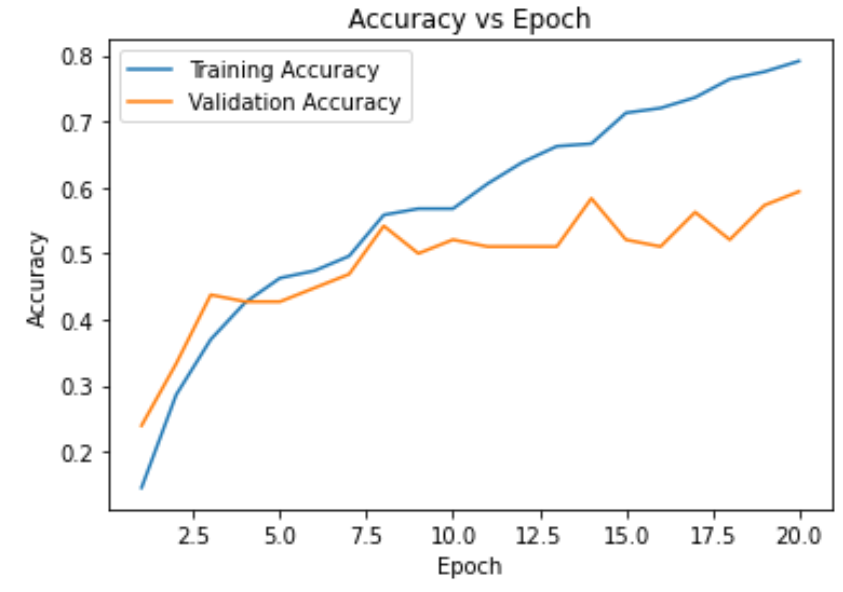
\includegraphics[width=2in, height = 1in]{12} \\ \hline
			
		\end{tabular}
	\end{center}
\end{table}

We performed data augmentation on our images and ran the model a second time to see if this would reduce the overfitting. For the Resnet model, the overfitting was significantly less; accuracy and loss were much closer between the training and validation sets. Overall model accuracy improved as well, with a 6.85\% increase in final validation accuracy. Overfitting was also reduced for the CvT model as well; the accuracy and loss were slightly closer between the training and validation sets. However, the validation loss of the CvT model still increased through training and ended up having a lower overall accuracy, decreasing by 9.37\% after data augmentation. 

\FloatBarrier
\subsection{Overall Highest Validation Accuracy of Models}

\begin{tabular}{|p{1.3in}|p{1.3in}|p{1.3in}|p{1.3cm}|}
	\hline 
	\rule{0pt}{20pt}
	& ResNet-50 & ViT & CVT \\
	\hline 
	\rule{0pt}{20pt}
	Without Augmentation & 35.42\% & 100\% & 68.75\% \\
	\hline 
	\rule{0pt}{20pt}
	With Augmentation & 42.27\% & 100\% & 59.38\% \\
	\hline
\end{tabular}
	
\section{Conclusions}

Image classification is a classic deep learning problem that has a multitude of practical applications. In this study we used three different models (ResNet50, ViT, and CVT) both with, and without data augmentation, in order to determine which would be most beneficial to a company like Match Group where the accurate classification of travel images could vastly improve their service.

While our results suggest that ViT was the best performing model, the fact that it achieved 100\% validation accuracy both with and without augmentation is somewhat suspect. This leads us to believe that the data augmentation failed to adequately address the overfitting issue. This conclusion is supported by the fact that the validation accuracy of CvT actually decreased by a significant margin after applying the transformations. All of the selected models have been known to perform well on similar tasks, so despite our results we still believe these models can classify similar images with a high degree of accuracy, however, in order to draw more concrete conclusions, similar investigations with larger datasets and more computational power appear to be necessary.

\section{Future Directions}

With these results in mind, we see a few paths forward in order to get better performance out of these models, or any other model individuals might choose to look at in the future.
As we know, a model is only as good as the data that you feed it. We believe that by utilizing a larger dataset we could have addressed some of the overfitting issues. Even when accounting for the data augmentation, there were far fewer images in our dataset than many other similar studies. Implementing dropout is another method to combat overfitting that we believe shows promise.

All of our models were pre-trained, so utilizing models that are not pre-trained, and comparing their performance is something we would want to try in the future.

Additionally, due to computational restraints, a lot of data was lost during the resizing of our images, however, if a large company or research group were to utilize our findings as a basis for further research, we believe

\nocite{Dosovitskiy}
\nocite{He}
\nocite{Wu}
\nocite{cvt}
\nocite{vit}
\nocite{resnet}
\printbibliography



\end{document}